% !TeX root = ../index.tex
\chapter{Object Oriented PHP \& MySQL}
\graphicspath{{5-oophp-mysql/images/}}

\section{Exercise 1}

\url{https://intweb.bucks.ac.uk/~21606555/oos/5-oophp-mysql/index.php}

\captionsetup{type=figure}\captionof{figure}{class\_lib.php}
\subfile{pyg/src/5-oophp-mysql/class_lib}

\clearpage
\captionsetup{type=figure}\captionof{figure}{index.php}
\subfile{pyg/src/5-oophp-mysql/index}

\begin{figure}[H]
  \caption{Result}
  \centering
  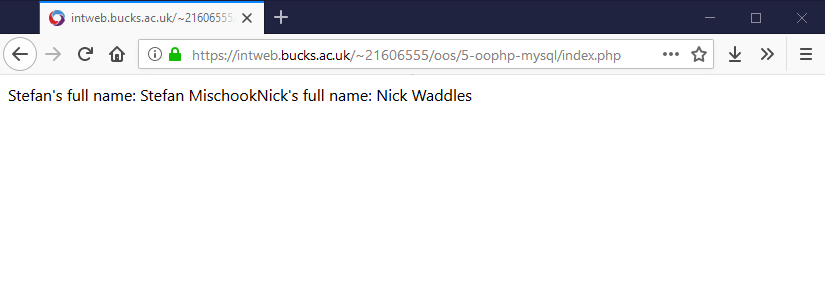
\includegraphics[width=\textwidth]{ex1}
\end{figure}

\section{Exercise 2}

\begin{figure}[H]
  \caption{Test table created}
  \centering
  \includegraphics[width=\textwidth]{ex2}
\end{figure}

\section{Exercise 3}

\begin{figure}[H]
  \caption{Added row to table}
  \centering
  \includegraphics[width=\textwidth]{ex3}
\end{figure}

\section{Exercise 4}

\begin{figure}[H]
  \caption{Searching for Bugs Bunny}
  \centering
  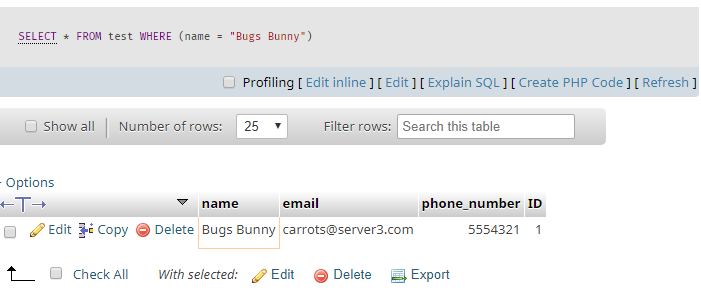
\includegraphics[width=\textwidth]{ex4}
\end{figure}

\section{Exercise 5}

\begin{figure}[H]
  \caption{Adding more rows to test table}
  \centering
  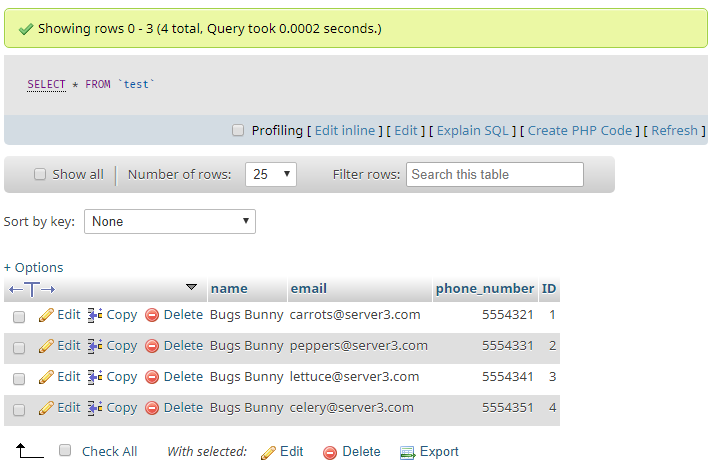
\includegraphics[width=\textwidth]{ex5}
\end{figure}

\section{Exercise 6}

\begin{figure}[H]
  \caption{Searching for all Bugs Bunny}
  \centering
  
\includegraphics[width=\textwidth]{ex6}
\end{figure}

\section{Exercise 7}

\begin{figure}[H]
  \caption{Deleting a row}
  \centering
  \includegraphics[width=\textwidth]{ex7}
\end{figure}

\section{Exercise 8}

\begin{figure}[H]
  \caption{Modifying cells in tables}
  \centering
  \includegraphics[width=\textwidth]{ex8}
\end{figure}
